\hypertarget{kolejka_8cpp}{\section{Dokumentacja pliku kolejka.\-cpp}
\label{kolejka_8cpp}\index{kolejka.\-cpp@{kolejka.\-cpp}}
}


Zawiera definicje metod klasy \hyperlink{class_kolejka}{Kolejka}.  


{\ttfamily \#include \char`\"{}kolejka.\-hh\char`\"{}}\\*
Wykres zależności załączania dla kolejka.\-cpp\-:\nopagebreak
\begin{figure}[H]
\begin{center}
\leavevmode
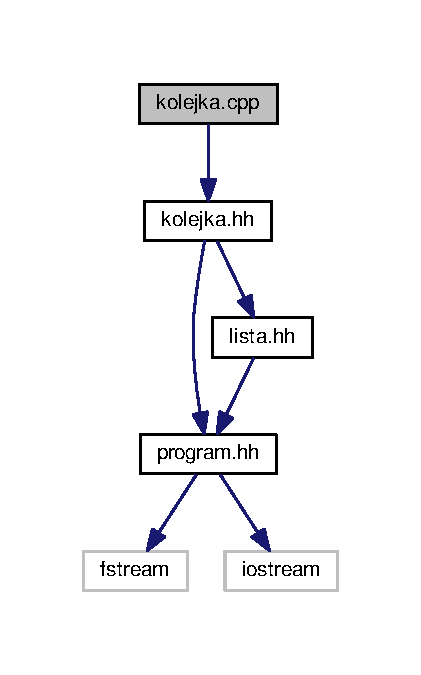
\includegraphics[width=202pt]{kolejka_8cpp__incl}
\end{center}
\end{figure}
